\documentclass[11pt,a4paper]{article}
\usepackage[utf8]{inputenc}
\usepackage[T1]{fontenc}
\usepackage[a4paper, left=2cm, right=2cm, top=3cm, bottom=2cm]{geometry}

\begin{document}

\title{Robot, Explain Yourself\\
Enhancing Human-Robot Communication with Large Language Models}
\author{Willem Adnet}
\date{\today}
\maketitle

\begin{abstract}
This report presents the design and implementation of a system for enhancing human-robot interaction by enabling a robot to explain its decisions, particularly those related to low-level perception data, through natural language using a Large Language Model (LLM).
The project explores current methodologies, builds an integration framework, fine-tunes an LLM, and validates the system through user evaluations.
\end{abstract}

\tableofcontents
\newpage

\section{Introduction}

The integration of artificial intelligence with robotics has opened new frontiers in human-robot interaction (HRI). As robots become increasingly autonomous and deployed in complex real-world environments, the need for transparent and interpretable decision-making becomes paramount.
This project addresses the challenge of making robotic systems more explainable by leveraging Large Language Models (LLMs) to translate low-level sensor data and perception information into natural language explanations.

\subsection{Problem statement}

Modern robots operate using complex algorithms that process vast amounts of sensor data to make navigation and behavioral decisions.
However, these decisions often remain opaque to human users, creating a barrier to trust and effective collaboration.
The challenge lies in bridging the gap between machine perception and human understanding.

The primary goal is to develop an AI-powered robot capable of evaluating its past decisions, particularly when revisiting locations.
For example, the robot should be able to explain: "I recognize this area—I previously visited it on [date/time] and made a certain decision."
If the environment has changed since the last visit, the robot should update its reasoning to reflect the new context, rather than relying solely on prior experiences.

\subsection{Objectives}

This project aims to:
\begin{itemize}
    \item Design a framework for integrating LLMs with robotic perception systems
    \item Develop a prototype system that can explain robot path decisions in natural language
    \item Evaluate the effectiveness of LLM-generated explanations in enhancing human understanding
    \item Assess the impact on user trust and satisfaction in human-robot interactions
\end{itemize}

\section{Literature Review}

This literature review summarizes the current state of technologies and methodologies in human-robot communication, focusing particularly on interpretability and explainability of low-level perception information, and the associated challenges and opportunities in making robotic behavior understandable to human users.

\subsection{Human-Robot Communication Technologies}

Current approaches to human-robot communication span multiple modalities including speech, gesture, and visual interfaces.
Recent advances in dialogue management systems have shown promise in creating more natural interactions \cite{dialogue_management_2023}.

\subsection{Explainable AI in Robotics}

The field of explainable AI (XAI) has gained significant attention, particularly in safety-critical applications.
Trust calibration and explanation specificity have emerged as key factors in building reliable human-robot relationships \cite{trust_explainable_robots_2020}.

\subsection{Large Language Models in Robotics}

Recent work has explored the integration of LLMs with robotic systems for various tasks including instruction following, task planning, and human-robot dialogue.
The emergence of foundation models has opened new possibilities for natural language interfaces in robotics \cite{llm_robotics_2024}.

\subsection{Challenges and Opportunities}

Key challenges include real-time processing constraints, the interpretability gap between sensor data and natural language, and the need for context-aware explanations.
Opportunities exist in leveraging pre-trained language models and developing domain-specific fine-tuning approaches.

\section{Framework Design}

\subsection{Architecture Overview}

The proposed framework integrates three main components:
\begin{enumerate}
    \item \textbf{Perception Processing Layer}: Handles sensor data aggregation and context extraction
    \item \textbf{LLM Integration Layer}: Manages prompt generation and response processing
    \item \textbf{Human Interface Layer}: Provides natural language interaction capabilities
\end{enumerate}

\begin{center}
    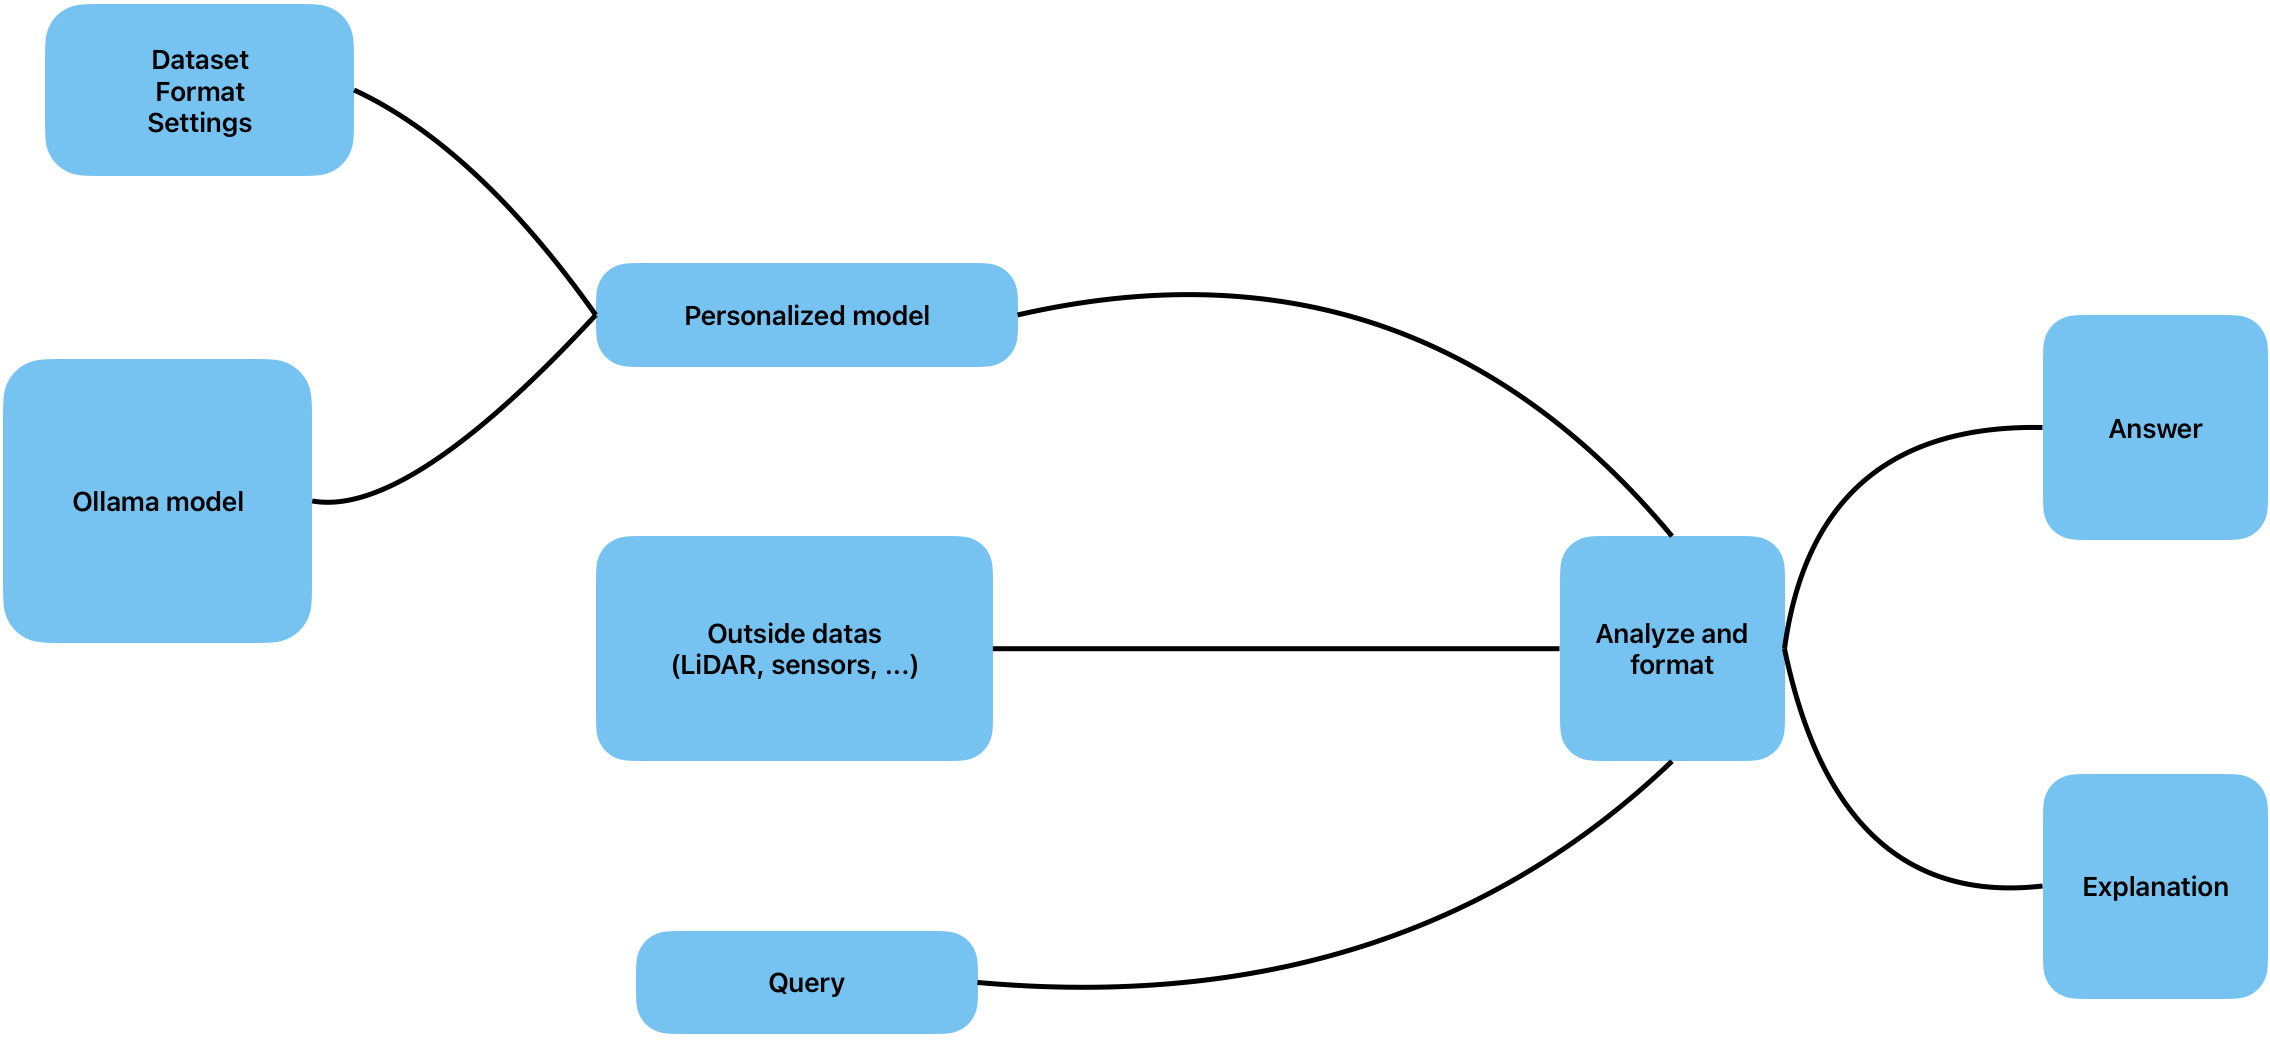
\includegraphics[scale=0.45]{figures/Model-HCI.png}
\end{center}

\subsection{Installation of the Project}

The project is designed to be easily deployable on any computer with minimal setup requirements. The following prerequisites are needed:

\begin{itemize}
    \item \textbf{Python 3.8+} (recommended: Python 3.11)
    \item \textbf{Ollama} - Local LLM server for model hosting
    \item \textbf{llama3.2} model or compatible LLM model
    \item \textbf{make} (optional, for automation)
    \item \textbf{git} for repository cloning
\end{itemize}

\subsubsection{Step-by-Step Installation Process}

\textbf{1. Repository cloning}

The project can be obtained from the GitHub repository:

\begin{verbatim}
    git clone https://github.com/Vlor999/HCI.git
    cd HCI
\end{verbatim}

\textbf{2. Ollama installation and setup}

Ollama serves as the local LLM server, providing the computational backend for natural language processing:

\begin{itemize}
    \item Download and install Ollama from \texttt{https://ollama.com/download}
    \item Start the Ollama server: \texttt{ollama serve}
    \item Pull the required model: \texttt{ollama pull llama3.2} (or any other model)
\end{itemize}

\textbf{3. Project environment setup}

The project uses automated setup through make commands:

\begin{verbatim}
    make init
    make install
\end{verbatim}

This process creates the necessary directory structure and installs Python dependencies in a virtual environment.

\textbf{4. Optional code formatting}

For development consistency:

\begin{verbatim}
    make format
\end{verbatim}
But if you also want to stay consistent with the all code you have to run the following command :
\begin{verbatim}
    pre-commit install
\end{verbatim}
Like that for the next commit that you'll do everything will be checked before you submit it.

\subsection{System execution}

\subsubsection{Running the Application}

The system can be launched using either automated make commands or direct Python execution:

\begin{verbatim}
    make run
\end{verbatim}

or manually:

\begin{verbatim}
    .venv/bin/python main.py
\end{verbatim}

Obviously you can add some CLI commands and if you are into the current env you can simply run :

\begin{verbatim}
    python main.py
\end{verbatim}

If you want to know all the commands that can be used try the help CLI argument.

\subsubsection{Testing Framework}

The project includes comprehensive testing capabilities:

\begin{verbatim}
    make test
\end{verbatim}

For coverage analysis with HTML reporting:

\begin{verbatim}
    make coverage
\end{verbatim}

The coverage report can be viewed by opening \texttt{htmlcov/index.html} in a web browser.

\subsection{Data flow and processing pipeline}

The system processes robot perception data through a structured pipeline:
\begin{itemize}
    \item Environmental/Weather context extraction from sensor readings
    \item Path analysis and decision point identification
    \item Prompt template generation with structured information
    \item LLM query processing and response generation
    \item Natural language explanation delivery to users
\end{itemize}


\subsection{Project structure and organization}

The framework follows a modular architecture with clear separation of concerns:

\begin{verbatim}
    src/           # Source code modules
    tests/         # Unit tests and test data
    data/          # Example path scenarios (JSON)
    log/           # Conversation logs (Markdown)
    doc/           # Documentation and roadmap
    evaluation/    # Evaluation scripts and results
    Makefile       # Automation commands
    requirements.txt # Python dependencies
\end{verbatim}

\subsection{Usage workflow}

The typical user interaction follows this pattern:
\begin{enumerate}
    \item The system displays current robot path and environmental context
    \item Users can ask multiple questions about path decisions and conditions
    \item The LLM processes queries and generates contextual explanations
    \item Sessions are terminated with \texttt{exit} or \texttt{quit} commands
    \item Conversation logs are automatically saved in Markdown format in the \texttt{log/} directory
\end{enumerate}

\subsection{Configuration and customization}

The system supports various customization options:

\begin{itemize}
    \item \textbf{Path scenarios}: Edit \texttt{data/paths.json} to add or modify navigation scenarios
    \item \textbf{LLM models}: The model name can be changed in the source code for different LLM variants
    \item \textbf{Logging}: Conversation logs are automatically generated and stored for analysis
\end{itemize}

\subsection{Technical requirements}

The framework is designed with several technical requirements in mind.
It must support real-time processing to enable interactive use and immediate responses to user queries.
The architecture should remain modular to facilitate adaptation across different robot platforms and allow for future extensions.
Scalability is also essential, ensuring that the system can handle a variety of explanation types and increasing complexity as needed.

\subsection{Troubleshooting and common issues}

When deploying the system, several common issues may arise. First, it is important to ensure that the Ollama server is running by verifying that the \texttt{ollama serve} command is active and that the required model has been properly pulled.
Port conflicts can also occur, as only one Ollama server instance should be running on port 11434 at any given time. Additionally, the Python environment must be correctly set up, make sure that the virtual environment (\texttt{.venv}) is properly activated before running any Python scripts.
Finally, confirm that the necessary large language model (LLM) is downloaded and accessible to avoid runtime errors related to model availability.
\subsection{Integration Capabilities}

\section{LLM Customization}

\subsection{Model selection and comparison}

The project employed multiple LLM architectures to determine which one provided the most accurate answers while also offering the most comprehensive explanations.
The LLM used during this project are the next ones :
\begin{table}[ht]
    \centering
    \begin{tabular}{|l|l|l|}
        \hline
        \textbf{Model}      & \textbf{Size} & \textbf{Performance} \\
        \hline
        Llama 3.2           & 2.0 GB        & Baseline performance \\
        nous-hermes2:latest & 6.1 GB        & small model that explain lightly \\
        deepseek            & 8.1 GB        & Good reasoning, efficient and clear\\
        qwen3:30b-a3b       & 18 GB         & big model that provides good answers but take some time \\
        \hline
    \end{tabular}
    \caption{LLM model comparison}
\end{table}

\subsection{Prompt engineering}

Effective prompt design proved crucial for generating relevant explanations. The system uses structured prompts that include:
\begin{itemize}
    \item Environmental context and sensor readings
    \item Historical path information
    \item User questions and interaction history
    \item Domain-specific constraints and objectives
    \item Additional datas provided by the human or captors
    \item Typical question/answer results
\end{itemize}

\subsection{Fine-tuning approach}

The customization process involved:
\begin{itemize}
    \item Dataset creation with robot-specific scenarios
    \item Prompt template
    \item Response quality evaluation and iteration
    \item Integration with robot perception systems
\end{itemize}

\section{Human-Robot Interaction Prototype}

\subsection{System implementation}

The prototype system was implemented using Python with the following key components:
\begin{itemize}
    \item \textbf{Path processing module}: Handles environmental data and context extraction
    \item \textbf{LLM interface}: Manages communication with local Ollama server
    \item \textbf{Conversation manager}: Maintains interaction history and context
    \item \textbf{User interface}: Provides command-line and potential interaction
\end{itemize}

\subsection{Core features}

The implemented system supports:
\begin{itemize}
    \item Interactive questioning about robot path decisions
    \item Real-time explanation generation
    \item Context-aware responses based on environmental conditions
    \item Conversation logging and history management
    \item Multiple scenario support for testing and evaluation
\end{itemize}

\subsection{Technical architecture}

The system architecture follows a modular design:
\begin{itemize}
    \item \texttt{robotPathExplanation.py}: Main application logic
    \item \texttt{path.py}: Data structures for path and environmental information
    \item \texttt{llmModel.py}: LLM integration and prompt management
    \item \texttt{conversationLogger.py}: Interaction recording and analysis
\end{itemize}

\subsection{Usage scenarios}

The prototype supports various interaction scenarios:
\begin{enumerate}
    \item Path selection queries (e.g., "Which path should I take if I want the easiest route?")
    \item Safety-related questions (e.g., "I have a heavy load. Which path is safest?")
    \item Time-constrained decisions (e.g., "I am in a hurry but want to avoid danger")
    \item Real-time updated decision (e.g., "Which path should i took according to the new datas that I provided ?")
\end{enumerate}

\section{Evaluation}

\subsection{Evaluation methodology}

The system evaluation employed multiple approaches:
\begin{itemize}
    \item \textbf{Automated testing}: Unit tests for core functionality and edge cases. Run when you commit something
    \item \textbf{Explanation quality assessment}: Keyword matching and semantic similarity analysis
    \item \textbf{User study design}: Interactive scenarios with human participants
    \item \textbf{Performance metrics}: Response time, accuracy, and user satisfaction measures (not really efficient but look if the answer makes sense)
\end{itemize}

\subsection{Quantitative results}

The evaluation framework assessed explanations based on:
\begin{itemize}
    \item Keyword coverage score (target: $\geq$ 75\%)
    \item Factual accuracy in decision reasoning
    \item Consistency across similar scenarios
\end{itemize}

\subsection{Qualitative findings}

Key observations from the evaluation include:
\begin{itemize}
    \item Users appreciated natural language explanations
    \item Context-aware responses significantly improved user understanding
    \item Explanation quality varied with environmental complexity
    \item Interactive questioning enhanced user engagement and trust
\end{itemize}

\subsection{Limitations and challenges}

Identified limitations include:
\begin{itemize}
    \item Computational overhead for real-time processing
    \item Occasional over-fitting in response patterns
    \item Context window limitations for extended conversations
    \item Need for domain-specific fine-tuning for optimal performance
\end{itemize}

\section{Conclusion}

\subsection{Summary of contributions}

This project successfully demonstrated the feasibility of using Large Language Models to enhance human-robot communication through natural language explanations of robotic decisions.
Key contributions include:

\begin{itemize}
    \item A novel integration framework for LLMs in robotic explanation systems
    \item A working prototype that translates low-level perception data into natural language (theoradicaly)
    \item Empirical evaluation demonstrating improved user understanding and engagement
    \item Open-source implementation available for further research and development
\end{itemize}

\subsection{Impact and implications}

The work addresses a critical gap in human-robot interaction by making robotic decision-making more transparent and interpretable.
This has implications for:
\begin{itemize}
    \item Increased user trust in autonomous systems
    \item Enhanced collaboration in human-robot teams
    \item Improved debugging and system maintenance
    \item Better user training and system adoption
\end{itemize}

\subsection{Future work}
Several directions for future research emerge from this work:
\begin{itemize}
    \item \textbf{Real-time integration :} Developing more efficient processing pipelines for live robot systems.
    \item \textbf{Multimodal explanations :} Incorporating visual and gestural explanation modalities.
    \item \textbf{Personalized explanations :} Adapting explanation style to individual user preferences.
    \item \textbf{Domain expansion :} Extending beyond path planning to other robotic decision domains.
    \item \textbf{Fine-tuning optimization :} We can develop robot-specific language models to improve performance, or we can directly train a robot to perform the exact task we are searching for.
\end{itemize}

\subsection{Final remarks}

The integration of Large Language Models with robotic systems represents a promising approach to bridging the communication gap between humans and machines. As LLM technology continues to advance, we can expect even more sophisticated and natural human-robot interactions, ultimately leading to more effective and trustworthy autonomous systems.
The open-source nature of this implementation encourages further research and development in this important area of human-robot interaction.


\bibliography{bibliography}
\bibliographystyle{plain}

\end{document}
